\section[Estrutura] {Estrutura}
\subsection{Conceito}

O robô será usado em bibliotecas para manipular os livros, assim precisa ser rápido, preciso e durável o suficiente para gerar real benefício. Para isso, será necessário uma estrutura que suporte as forças geradas pelo peso da payload e pela movimentação, sem danos ao robô ou aos livros.

Devido à aplicação e à forma de armazenamento dos livros, serão necessários três movimentos de translação: um paralelo ao comprimento da estante ( Que chamaremos de eixo “x”), um normal ao plano da estante (eixo “y”) e um paralelo à altura da estante (eixo “z”). Para movimentos de translação movidos por motores giratórios, tivemos as seguintes opções:

\begin{itemize}
\item{Correntes, Correias e Cabos}
\end{itemize}

Correntes são muito úteis para a transmissão de várias distâncias, além de muito baratas. Mas por não ser rígida, acaba por não apoiar a movimentação do robô, deixando-o instável. Por conta dessa instabilidade complexa de se tratar, essa opção foi descartada para o uso no projeto.  

\begin{itemize}
\item{Cremalheiras}
\end{itemize}

As cremalheiras são muito usadas em maquinário pesado. São rápidas, com precisão mediana e versáteis: podem ser usadas para movimentos horizontais e verticais. Contudo, movimentos verticais demandam uma estrutura bem mais robusta que aumentaria muito o peso do robô. Sendo assim, essa opção será usada no deslocamento em X, pois nas bibliotecas esse será o maior deslocamento, demandando assim, maior velocidade.

\begin{itemize}
\item{Fusos}
\end{itemize}

Fusos são muito utilizados desde CNC’s a Portões eletrônicos de garagem. São altamente precisos e resistentes, além de possuírem montagem e manutenção simples. Contudo, seu movimento é dependente do passo, o que pode colocar em cheque sua precisão ou o tempo de operação. Como a precisão vertical é a mais permissiva de erros em nosso projeto, optamos por essa solução para o deslocamento em Z, uma vez que o fuso pode ser empregado com um passo grande o suficiente para manter uma velocidade aceitável.

\begin{itemize}
\item{Atuadores Lineares}
\end{itemize}

Atuadores lineares podem ser usados apenas para pequenas distâncias, contudo são extremamente simples e compactos para pequenos movimentos que não requerem precisão. Assim, estes compõem a escolha para movimentos no eixo Y, que simplesmente servirão para trazer o ímã próximo o suficiente do livro para pegá-lo e então de volta para o apoio para o transporte da payload. Devido à pequena amplitude dos movimentos em Y, um atuador linear se torna uma boa opção para esse movimento.

\subsection{Materiais}

Como é um robô de dimensões relativamente grandes - aproximadamente do tamanho de uma pessoa, mas com leves solicitações, é interessante que seja feito com materiais leves e de baixo custo para que o tamanho da estrutura não traga muito mais esforços adicionais nem encarecer o projeto e construção do protótipo.Como cada parte sofre esforços e tem funções distintas, as escolhas de materiais para cada parte será:

\begin{itemize}
\item{Cases}
\end{itemize}

Os compartimentos onde os livros ficam guardados podem ser construídos em madeira, polímero ou metal. No caso de material não-magnético será necessário a aplicação de uma placa de ferro ou aço para que o eletroímã do atuador possa pegar o case com o livro. Visto que não há solicitações estruturais maiores que 2 kgf nos cases, decidimos pelo uso de madeira devido ao baixo peso, custo e facilidade de construção.

\begin{itemize}
\item{Pórtico}
\end{itemize}

O pórtico será feito com barras de alumínio 6063 estrutural de perfil 20x20 devido ao custo de aquisição e facilidade de montagem. O pórtico pode ser montado utilizando parafusos ou soldas, optamos por parafusos devido à praticidade e simplicidade desse método.

\begin{itemize}
\item{Fuso}
\end{itemize}

Fusos podem ser feitos de Alumínio ou aço. Fusos de Alumínio são recomendados para  baixas cargas e velocidades. O fuso será feito de aço porque é o material mais comum dos modelos disponíveis no mercado. A fabricação de um fuso é um processo de difícil execução, portanto a melhor opção é comprar um fuso.

\begin{itemize}
\item{Cremalheira e Engrenagem}
\end{itemize}

Existem duas opções no mercado, cremalheira de aço ou cremalheira de nylon com núcleo de aço. As cremalheiras de nylon são mais indicadas para máquinas leves com velocidades baixas assim como possuem um custo de aquisição menor se comparado às cremalheiras de aço. Por se tratar de uma aplicação leve, usaremos a cremalheira de nylon módulo1.

\subsection{Descrição do produto}

O robô consistirá de um atuador linear, apoiado em uma superfície plana de madeira, que se movimentará na direção vertical por meio de um fuso, e na direção horizontal por meio de uma cremalheira. A estante será subdividida de maneira padronizada, por meio de chapas de madeira, para acomodar cases dentro dos quais estarão os livros. Os cases não só abrigarão os livros como padronizarão o “tamanho” dos livros e suas orientações verticais, para melhor manuseio.

 A movimentação dos livros se dará por um poderoso eletroímã na ponta do atuador linear,que uma vez posicionado, será capaz de aderir-se ao case desejado, puxando-o para a superfície de madeira após o comando retrativo do atuador. Após a retirada do livro para a superfície, o robô se movimentará até uma mesa, posicionada ao lado da estante para a entrega do livro, onde o atuador empurrará o case e desativará seu eletroímã, deixando o livro no local da entrega. Um pórtico de alumínio estrutural garantirá as restrições necessárias para o engastamento do robô ao chão e restrição quanto aos possíveis momentos em torno dos eixos X e Z. A cremalheira será engastada ao chão, enquanto o pórtico também será apoiado em um trilho no topo da estante. Uma solução de baixo custo é o uso de um vergalhão de aço para o trilho.

Abaixo, encontram-se os cads realizados pela equipe de estruturas:
\begin{figure}[!h]		
\centering 
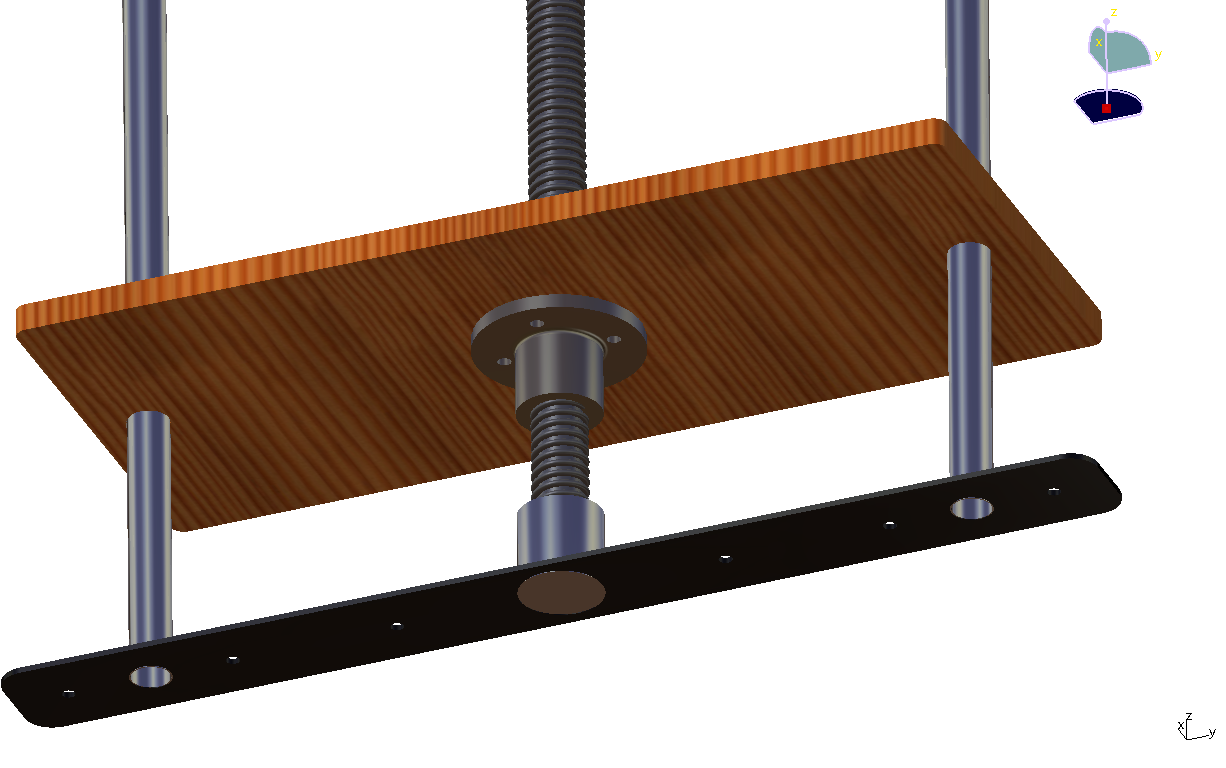
\includegraphics[scale=0.4]{figuras/screen_2}
\caption{Renderização do atuador vertical levemente estendido 40 mm}
\end{figure}
\FloatBarrier

\begin{figure}[!h]		
\centering
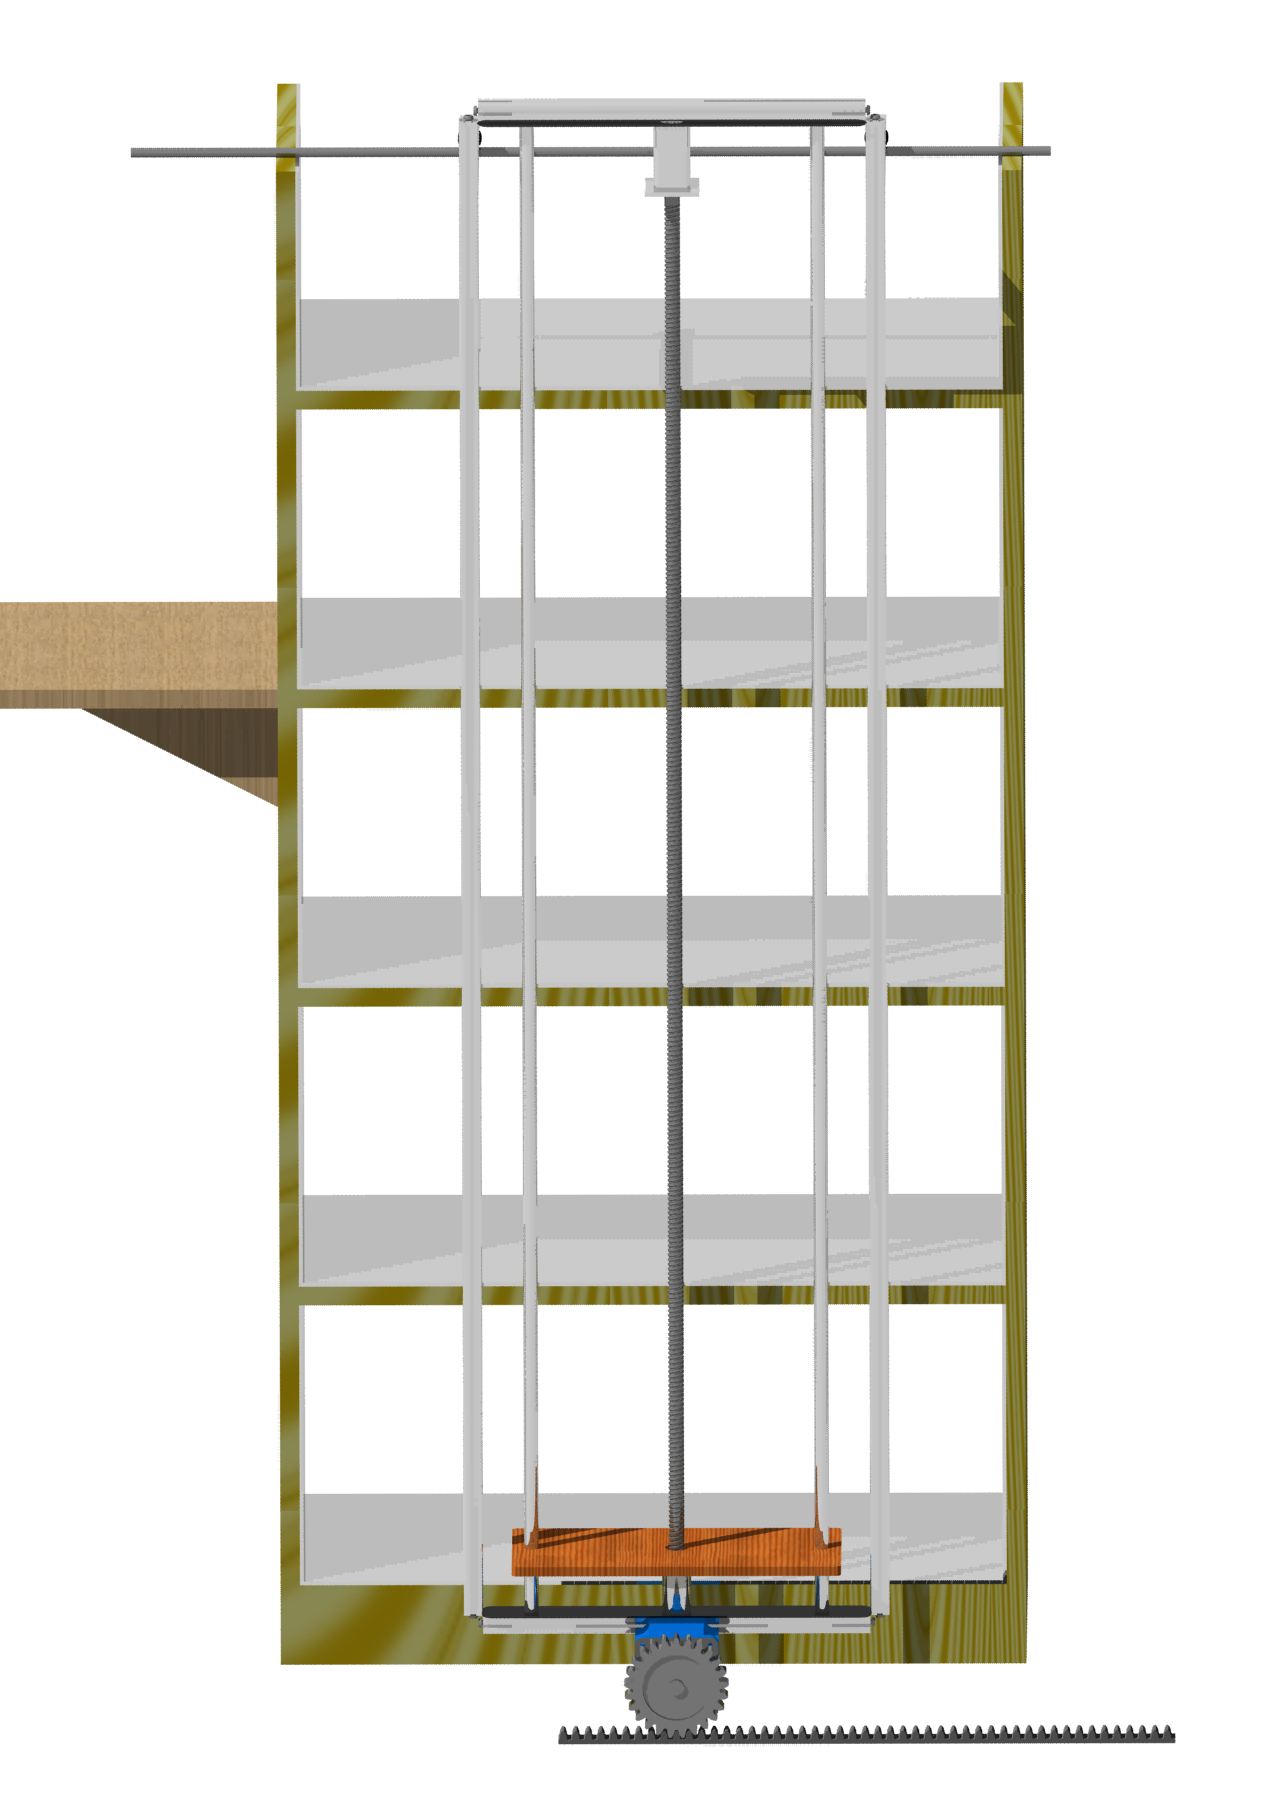
\includegraphics[scale=0.1]{figuras/render_frente}
\caption{Renderização do sistema completo-vista frontal}
\end{figure}
\FloatBarrier


\begin{figure}[!h]		
\centering
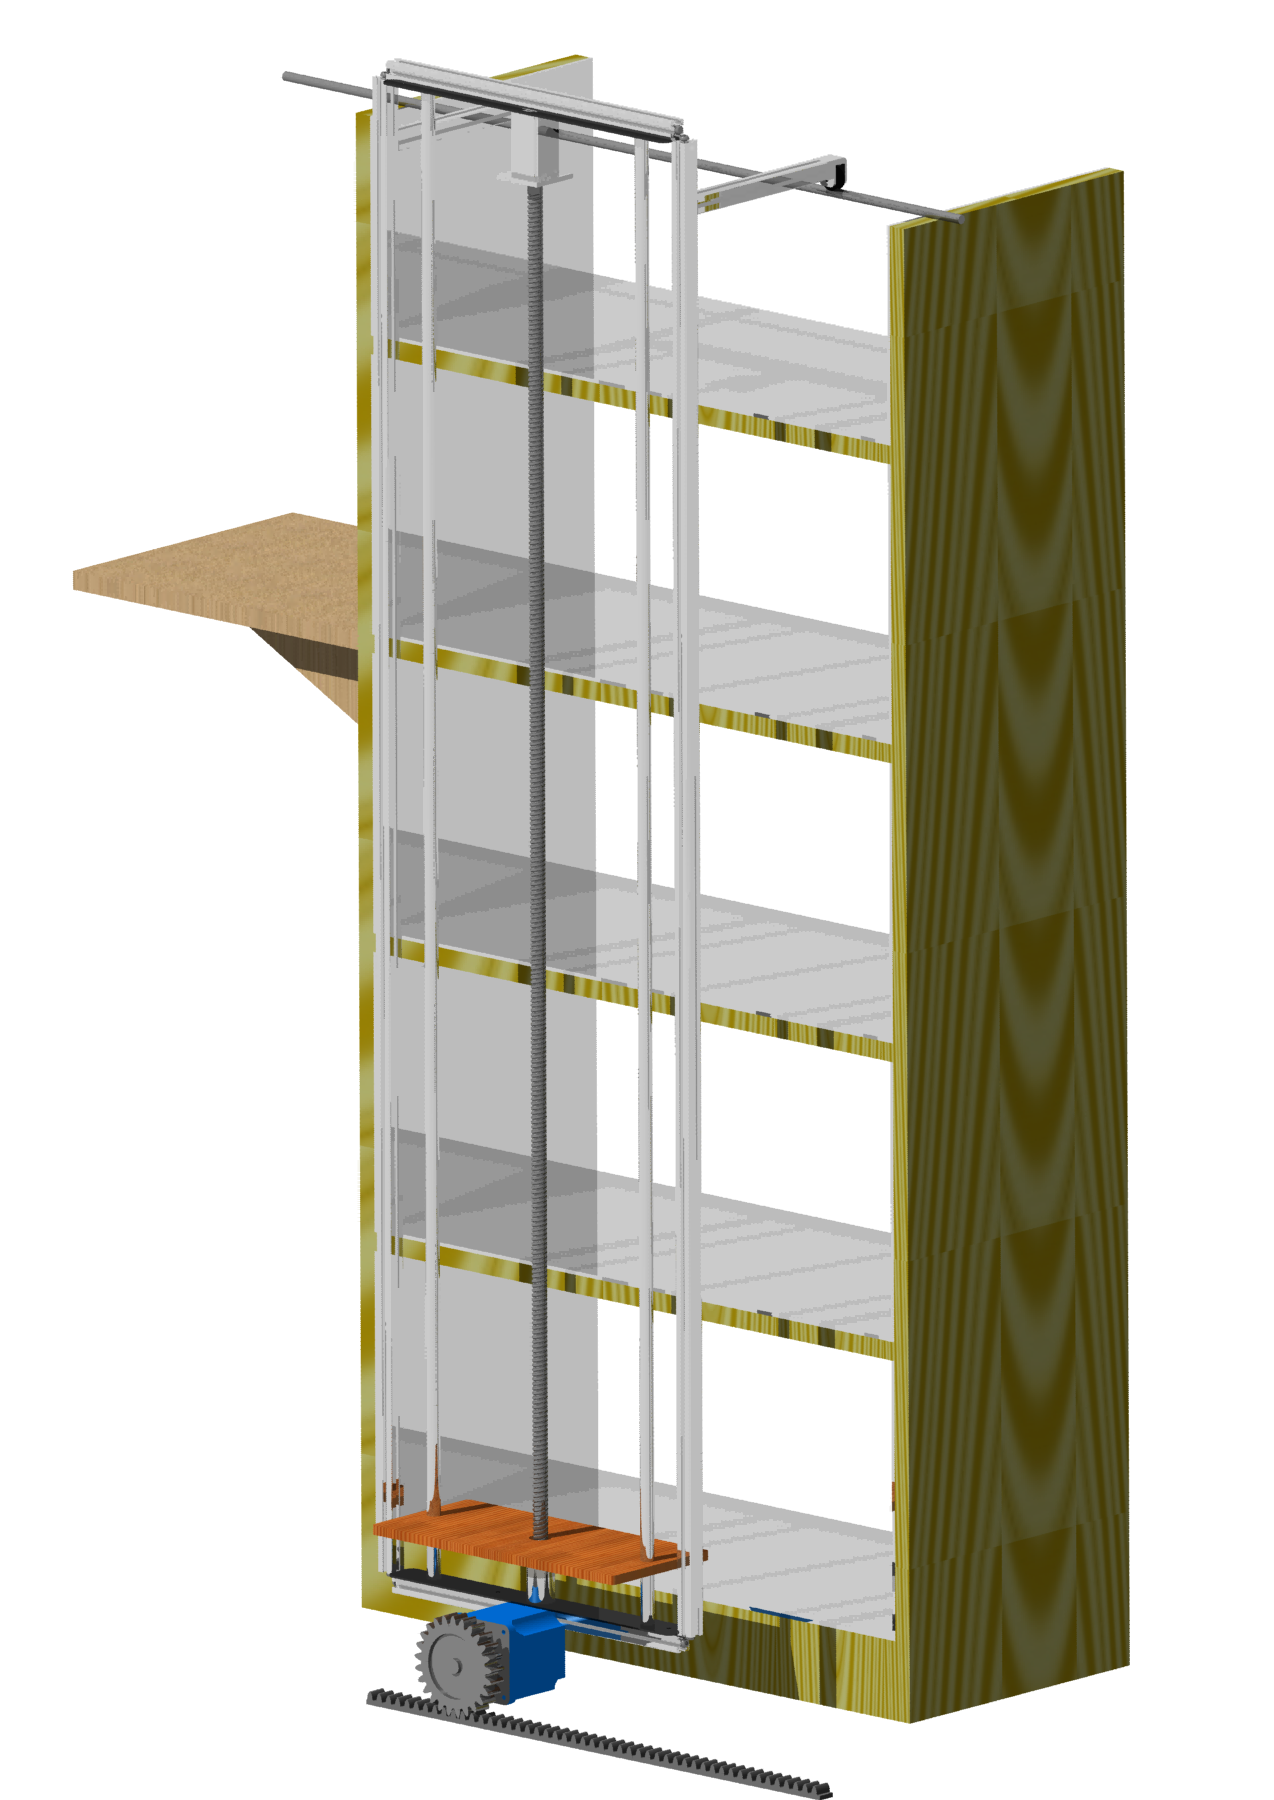
\includegraphics[scale=0.1]{figuras/render_full}
\caption{Renderização do sistema completo}
\end{figure}
\FloatBarrier
